\documentclass{standalone}
\usepackage{pgfplots}
\pgfplotsset{compat=newest}
\usepgfplotslibrary{ternary}
\begin{document}
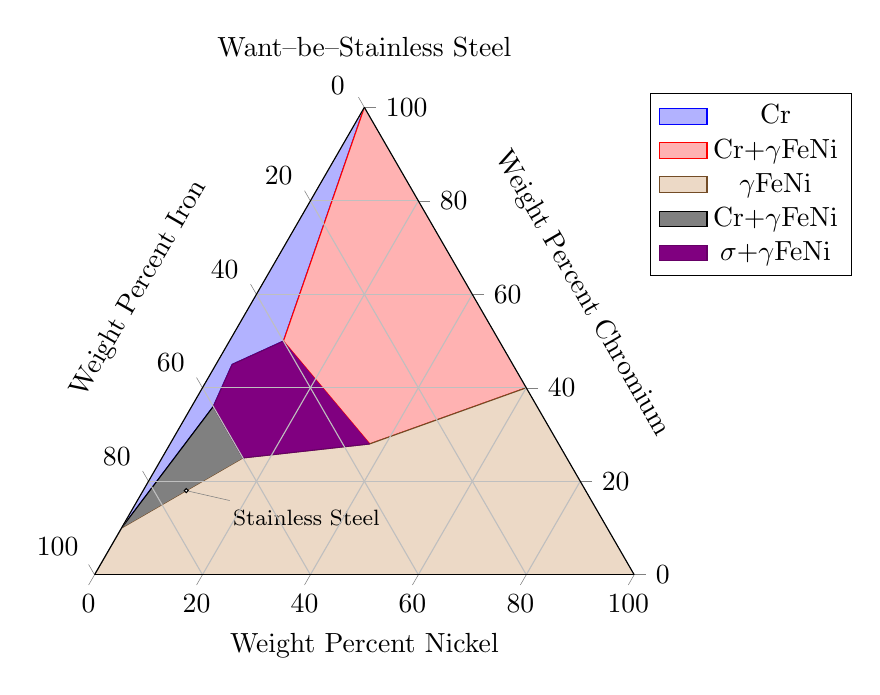
\begin{tikzpicture}
\begin{ternaryaxis}[
	title=Want--be--Stainless Steel,
	xlabel=Weight Percent Chromium,
	ylabel=Weight Percent Iron,
	zlabel=Weight Percent Nickel,
	label style=sloped,
	area style,
]
	\addplot3 table {
	A B C
	1 0 0
	0.5 0.4 0.1
	0.45 0.52 0.03
	0.36 0.6 0.04
	0.1 0.9 0
	};
	\addlegendentry{Cr}
	\addplot3 table {
	A B C
	1 0 0
	0.5 0.4 0.1
	0.28 0.35 0.37
	0.4 0 0.6
	};
	\addlegendentry{Cr+$\gamma$FeNi}
	\addplot3 table {
	0.4 0 0.6
	0.28 0.35 0.37
	0.25 0.6 0.15
	0.1 0.9 0
	0 1 0
	0 0 1
	};
	\addlegendentry{$\gamma$FeNi}
	\addplot3 table {
	0.1 0.9 0
	0.36 0.6 0.04
	0.25 0.6 0.15
	};
	\addlegendentry{Cr+$\gamma$FeNi}
	\addplot3 table {
	0.5 0.4 0.1
	0.45 0.52 0.03
	0.36 0.6 0.04
	0.25 0.6 0.15
	0.28 0.35 0.37
	};
	\addlegendentry{$\sigma$+$\gamma$FeNi}
	\node[inner sep=0.5pt,circle,draw,fill=white,pin=-15:\footnotesize Stainless Steel] 
	  at (axis cs:0.18,0.74,0.08) {};
	
\end{ternaryaxis}
\end{tikzpicture}
\end{document}
